\documentclass{article}
\usepackage{tikz}
\usetikzlibrary{positioning,calc,arrows.meta}
\usepackage{amsmath,amssymb}
\usepackage[margin=1in]{geometry}

\begin{document}

\begin{center}
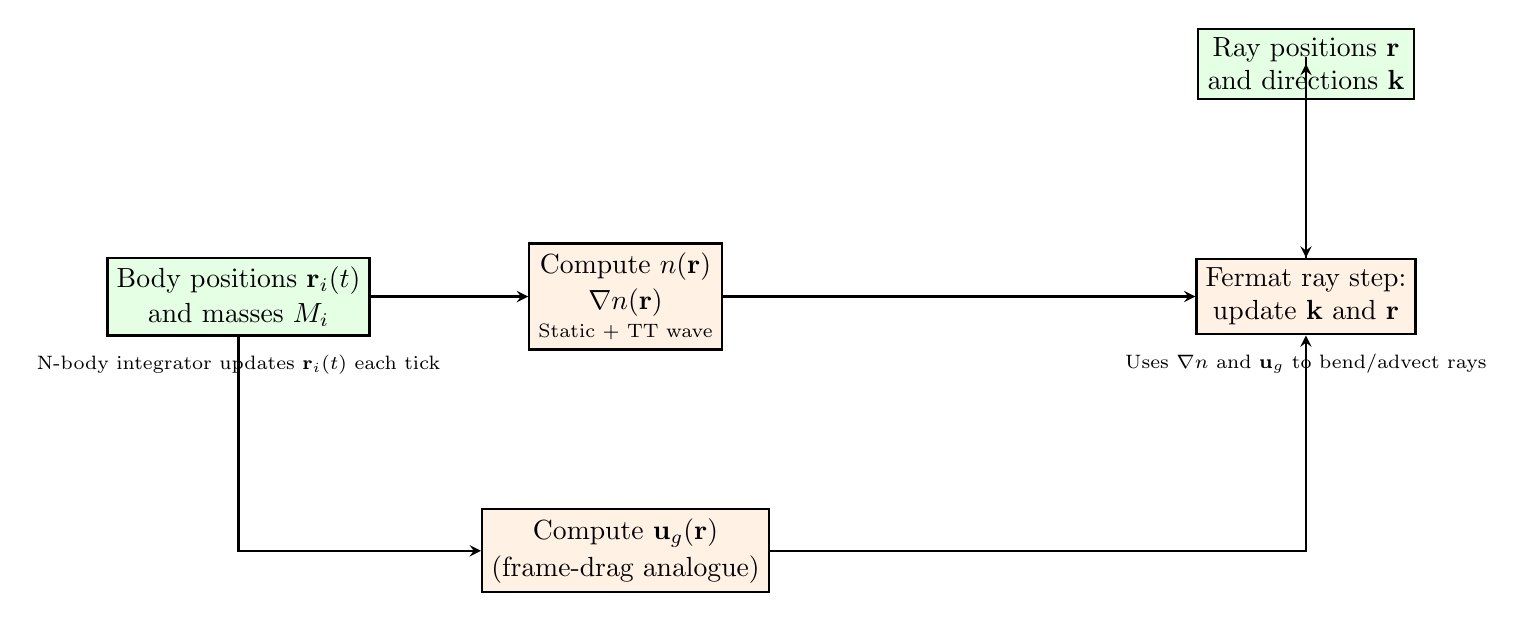
\begin{tikzpicture}[node distance=2cm,>=stealth,thick]
\tikzset{
  block/.style={rectangle, draw, rounded corners, align=center, fill=blue!10},
  data/.style={rectangle, draw, align=center, fill=green!10},
  calc/.style={rectangle, draw, align=center, fill=orange!10}
}

% Nodes (use shortstack for mixed math/text lines)
\node[data] (bodies) {\shortstack{Body positions $\mathbf{r}_i(t)$ \\
and masses $M_i$}};
\node[calc, right=of bodies] (nfield) {\shortstack{Compute $n(\mathbf{r})$ \\
$\nabla n(\mathbf{r})$ \\
{\scriptsize Static + TT wave}}};
\node[calc, below=of nfield] (flow) {\shortstack{Compute $\mathbf{u}_g(\mathbf{r})$ \\
(frame-drag analogue)}};
\node[calc, right=of nfield, xshift=4cm] (fermat) {\shortstack{Fermat ray step: \\
update $\mathbf{k}$ and $\mathbf{r}$}};
\node[data, above=of fermat] (rays) {\shortstack{Ray positions $\mathbf{r}$ \\
and directions $\mathbf{k}$}};

% Arrows
\draw[->] (bodies) -- (nfield);
\draw[->] (bodies) |- (flow);
\draw[->] (nfield) -- (fermat);
\draw[->] (flow) -| (fermat);
\draw[->] (rays) -- (fermat);
\draw[->] (fermat) |- (rays);

% Labels
\node[below=0.1cm of bodies] {\scriptsize N-body integrator updates $\mathbf{r}_i(t)$ each tick};
\node[below=0.1cm of fermat] {\scriptsize Uses $\nabla n$ and $\mathbf{u}_g$ to bend/advect rays};
\end{tikzpicture}
\end{center}

\end{document}
